%!TEX root = ../thesis.tex
\section{構造解析}
モータとリンクを繋ぐ板金部品の強度を,Inventorを用いた構造解析で確認した.本節では,特に強度が必要な肩部の部品について解析結果を述べる.肩部は,ヨー軸モータとピッチ軸モータを繋ぐ部品1,およびピッチ軸モータとリンクを繋ぐ部品2から構成される(図\ref{fig:shoulder}).

\begin{figure}[h]
  \centering
  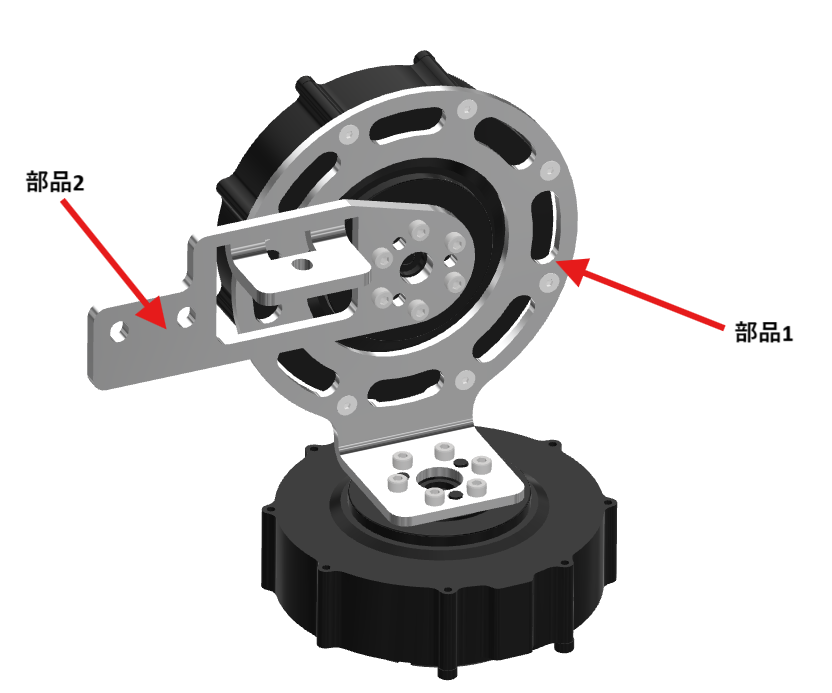
\includegraphics[width=10cm]{images/design/shoulder.png}
  \caption{Configuration of the shoulder components}
  \label{fig:shoulder}
\end{figure}

\subsection{部品1の構造解析}
部品1はアルミニウム合金(A5052)製で,ヨー軸モータの最大出力22Nm時に最大負荷を受ける.図\ref{fig:T3_40}に構造解析結果を示し,設計仕様を表\ref{tab:part1_spec}にまとめた.現設計では安全率が0.39で,強度が不足している.

\begin{figure}[h]
  \centering
  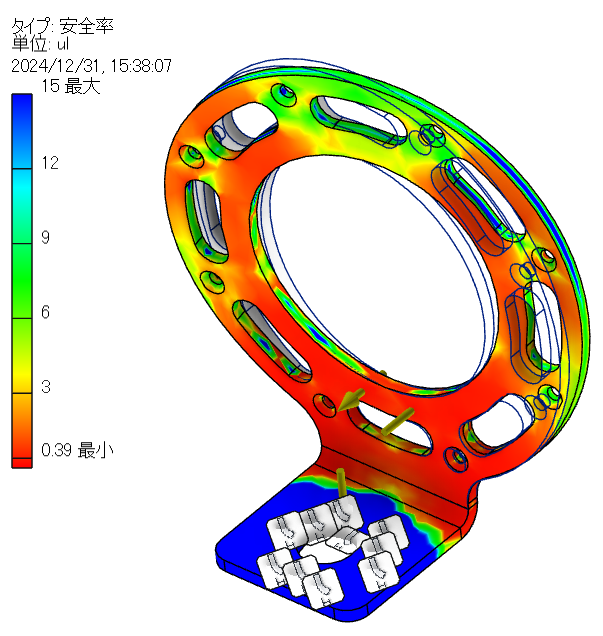
\includegraphics[width=6cm]{images/design/T3_40.png}
  \caption{Structural analysis results of Part 1 (current design)}
  \label{fig:T3_40}
\end{figure}

\begin{table}[h]
  \centering
  \caption{Specifications of Part 1 (current design)}
  \begin{tabular}{lc}
    \hline
    厚み & 3㎜ \\ 
    質量 & 43.6g \\ 
    安全率 & 0.39 \\ \hline
  \end{tabular}
  \label{tab:part1_spec}
\end{table}

厚みを5㎜に変更した場合,安全率が1.01に向上するが,質量が71.1gに増加する(図\ref{fig:T5},表\ref{tab:part1_spec_T5}参照).一方,厚みを3㎜のまま形状を最適化した結果,安全率は1.1に達し,質量を61.8gに抑えることができた(図\ref{fig:T3_80},表\ref{tab:part1_spec_T3_80}参照).最適化した形状を最終設計とする.

\begin{figure}[h]
  \centering
  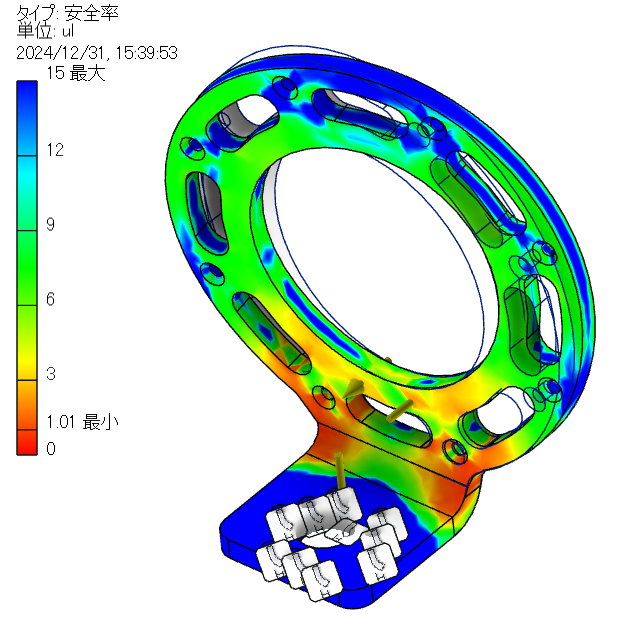
\includegraphics[width=6cm]{images/design/T5.png}
  \caption{Structural analysis results of Part 1 (thickness changed to 5mm)}
  \label{fig:T5}
\end{figure}

\begin{table}[h]
  \centering
  \caption{Specifications of Part 1 (thickness changed to 5mm)}
  \begin{tabular}{lc}
    \hline
    厚み & 5㎜ \\ 
    質量 & 71.1g \\ 
    安全率 & 1.01 \\ \hline
  \end{tabular}
  \label{tab:part1_spec_T5}
\end{table}

\begin{figure}[h]
  \centering
  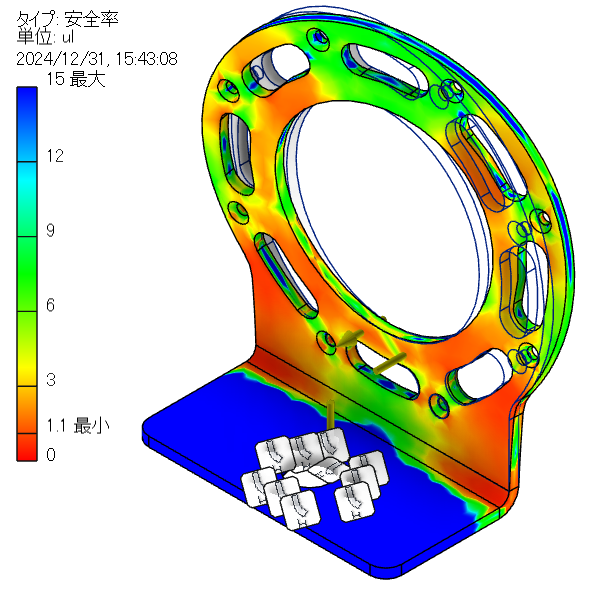
\includegraphics[width=6cm]{images/design/T3_80.png}
  \caption{Structural analysis results of Part 1 (shape optimized)}
  \label{fig:T3_80}
\end{figure}

\begin{table}[h]
  \centering
  \caption{Specifications of Part 1 (shape optimized)}
  \begin{tabular}{lc}
    \hline
    厚み & 3㎜ \\ 
    質量 & 61.8g \\ 
    安全率 & 1.1 \\ \hline
  \end{tabular}
  \label{tab:part1_spec_T3_80}
\end{table}

\subsection{部品2の構造解析}
部品2は,リンクを2方面から固定する形状を採用している(図\ref{fig:pitch}).最大負荷条件(22Nm)下での構造解析結果を図\ref{fig:pitch}に示す.現設計では安全率が0.47と低く,特に赤色部分に強度不足が確認される.

\begin{figure}[h]
  \centering
  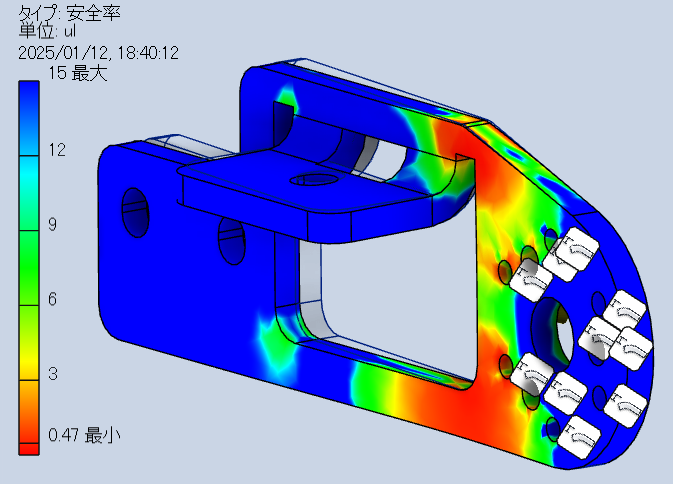
\includegraphics[width=6cm]{images/design/pitch.png}
  \caption{Structural analysis results of Part 2 (current design)}
  \label{fig:pitch}
\end{figure}

厚みを5㎜に変更した場合,安全率は0.58と改善するが依然不足している.構造解析を定格出力7.5Nmで実施した結果,安全率1.38が確認された(表\ref{tab:part2_spec}).定格条件下では強度が確保できるため,現設計を採用し,今後の形状改善を課題とする.

\begin{table}[h]
  \centering
  \caption{Specifications of Part 2 (after modification)}
  \begin{tabular}{lc}
    \hline
    厚み & 5㎜ \\ 
    質量 & 34.0g \\ 
    安全率 & 1.38 \\ \hline
  \end{tabular}
  \label{tab:part2_spec}
\end{table}

\newpage